\documentclass{article}

\usepackage[version=3]{mhchem} % Package for chemical equation typesetting
\usepackage{siunitx} % Provides the \SI{}{} and \si{} command for typesetting SI units
\usepackage{graphicx} % Required for the inclusion of images
\usepackage{natbib} % Required to change bibliography style to APA
\usepackage{amsmath} % Required for some math elements 
\usepackage{listings}

\setlength\parindent{0pt} % Removes all indentation from paragraphs

\renewcommand{\labelenumi}{\alph{enumi}.} % Make numbering in the enumerate environment by letter rather than number (e.g. section 6)

%\usepackage{times} % Uncomment to use the Times New Roman font

%----------------------------------------------------------------------------------------
%	DOCUMENT INFORMATION
%----------------------------------------------------------------------------------------

\title{Evolve a Species \\ COSC 343} % Title

\author{Steffan \textsc{Voges}} % Author name

\date{\today} % Date for the report

\begin{document}

\maketitle % Insert the title, author and date

% If you wish to include an abstract, uncomment the lines below
% \begin{abstract}
% Abstract text
% \end{abstract}

%----------------------------------------------------------------------------------------
%	SECTION 1
%----------------------------------------------------------------------------------------

\section{Description of Simulation}
\hspace{10 pt} The main method of the program takes in an unspecified number of arguments.  The first argument is the length of the world, and the second argument is the height of the world.  Optional flags can be added as well: '-i' requires user input in order to move to the next iteration; '-m' requires user input in order to do the next movement of either a creature or monster; and '-g' enables generational mode, in which creatures evolve and produce new generations.  Based on these inputs, a new world is instantiated, although no monsters are created yet. \\

\hspace{10 pt} After the world is instantiated, the program moves into the generations loop.  We repeat the following instructions 500 times: \\

\begin{description}
\item[Create a Generation]
If there are no people in the world (this happens when everyone has died either by eating a mushroom or touching a monster), we skip most of this method and only increment the generation by 1.  Otherwise, we create a new generation based on the fitness of each person from the old one.  The person with the highest fitness in the wold generation automatically moves on.  Then, we repopulate the world using tournament selection.  We pick a subset of the old generation, and pick the person with the highest fitness from this generation to be one parent.  We repeat the process with the other parent.  Then, using the chromosome from each parent, we create two new people by picking genes from the two parents at random and passing them on.  A mutation is introduced at a random point with a 1/7 chance.  We repeat the process above until we have repopulated our world with people. Note: I picked people both destructively and non-destructively, and explained the results below.
\item[Populate the World]
After creating all the necessary people, we must add monsters, mushrooms, and strawberries to our world as well.  These are added to random spots in the world, and the amount varies based upon the size of the array.  People are added as well if creating a new generation did not create enough people.
\item[Run Iterations]
Now that our world is populated, we run an iteration, in which each person does an action and each monster does a movement every second iteration.  First, a person must choose an action to do based on its surrounding state.  This is done by picking the best role (strawberry present, mushroom present, strawberry close, mushroom close, monster close, and person close) based on the weight of each role.  Out of all applicable roles, the role with the maximum weight is chosen, and it's action returned.  The person then executes the action returned.  If the action results in eating a strawberry, its energy will increase by 5; if it results in eating a mushroom, it dies; if it results in touching a monster, it dies as well.  Note that a person can be in the same square as a mushroom or strawberry and not eat it.  Each action that a person executes will decrease its energy level by 1- if it ends the turn with no energy, the person will die.  Next, monsters will do their turn if allowed.  They will only move towards the nearest person to them.
\end{description}

 
%----------------------------------------------------------------------------------------
%	SECTION 2
%----------------------------------------------------------------------------------------

\section{Data}

The following data is run on a 15 by 15 grid populated with 20 people, 20 strawberries, 5 monsters and 5 mushrooms.  Evolution is non-destructive, meaning that once two parents are selected they are not removed from the set of possible parents.

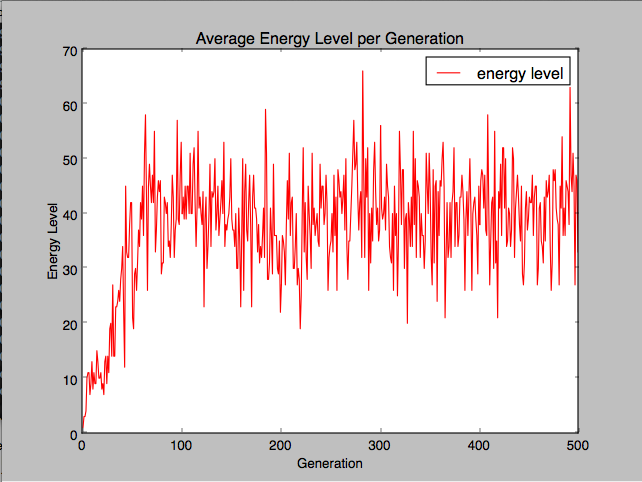
\includegraphics[width=1.25\textwidth]{15average_energy}
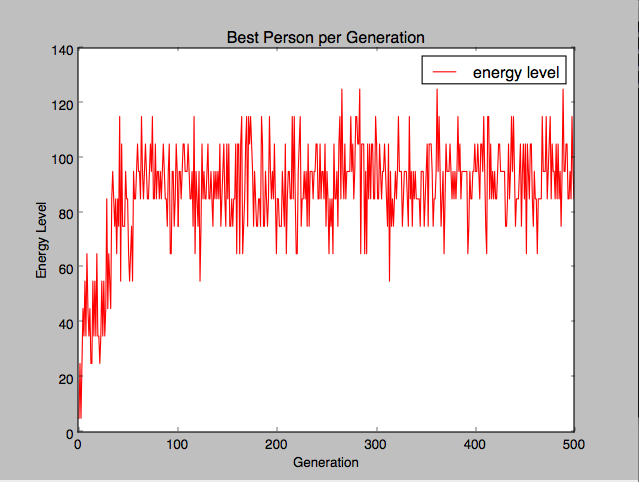
\includegraphics[width=1\textwidth]{15best_person}
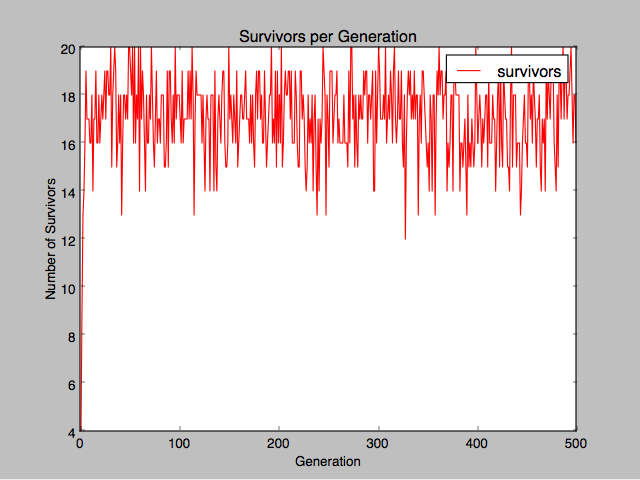
\includegraphics[width=1\textwidth]{15survivors}

The following data is run on a 40 by 40 grid populated with 50 people, 50 strawberries, 10 monsters and 10 mushrooms.  Evolution is non-destructive as well.  In the two cases below, creatures were initialized with 20 units of energy, but still had to go through 25 iterations, meaning they had to pick up at least 1 strawberry.

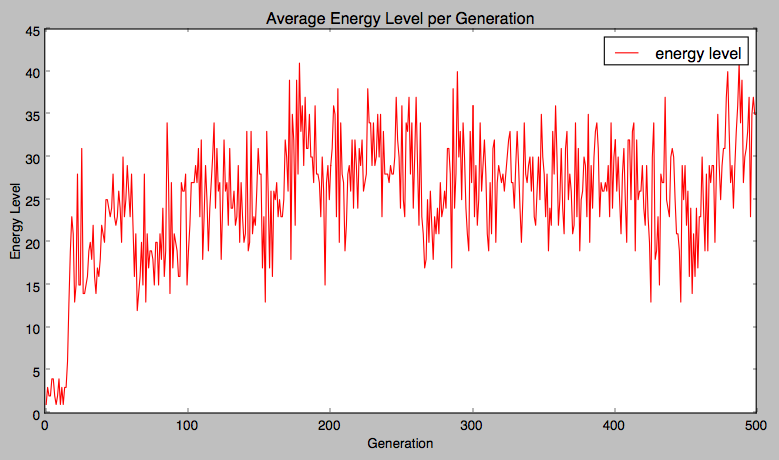
\includegraphics[width=1.25\textwidth]{40non_avg_energy}
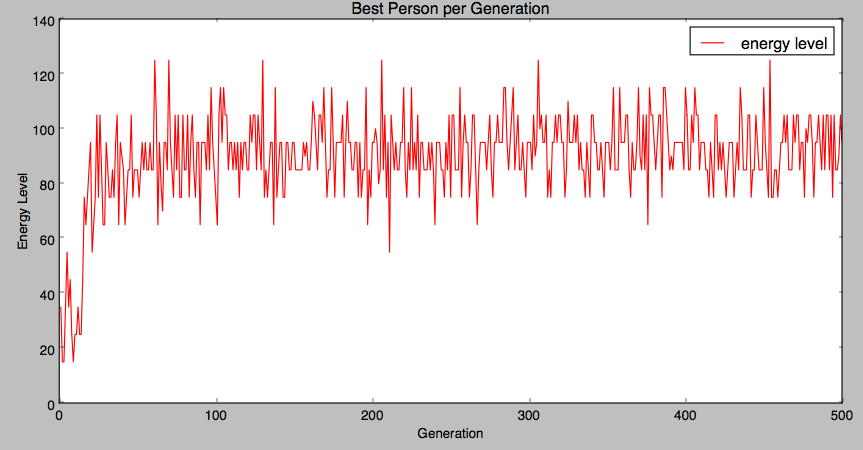
\includegraphics[width=1\textwidth]{40non_best}
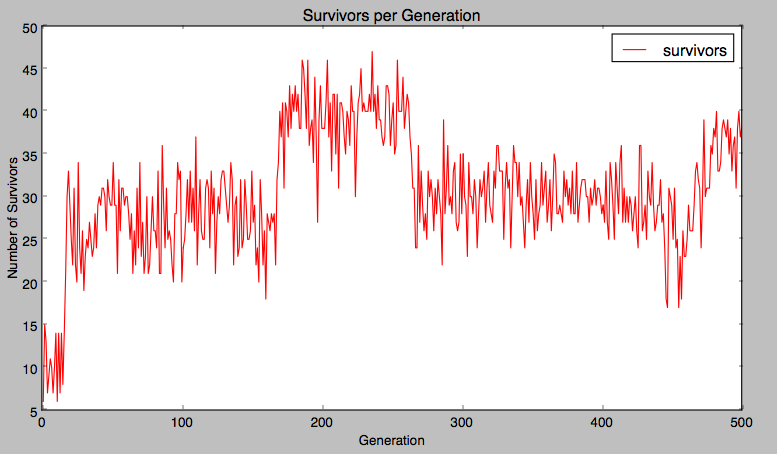
\includegraphics[width=1\textwidth]{40non_survivors}

The following data is run on a 40 by 40 grid populated with 50 people, 50 strawberries, 10 monsters and 10 mushrooms.  Evolution is destructive in this case, meaning that once parents are selected, they create two children and are then deleted from the set of possible parents.

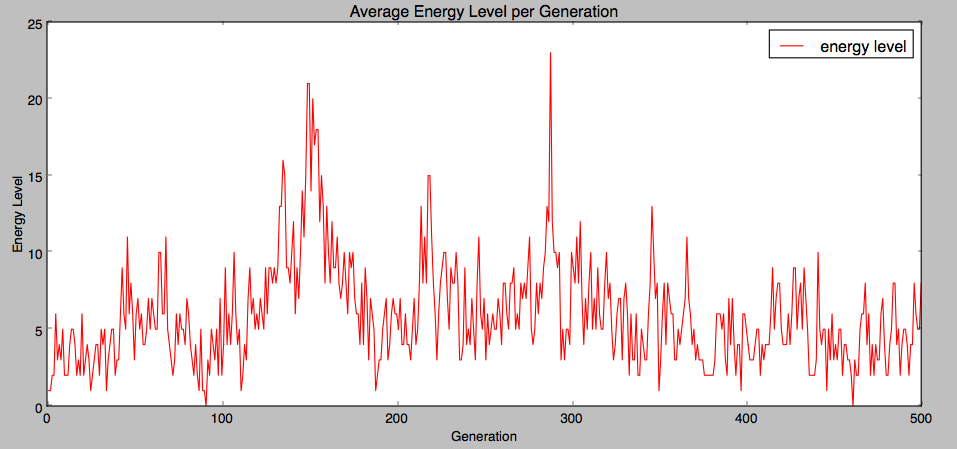
\includegraphics[width=1.25\textwidth]{40des_avg_energy}
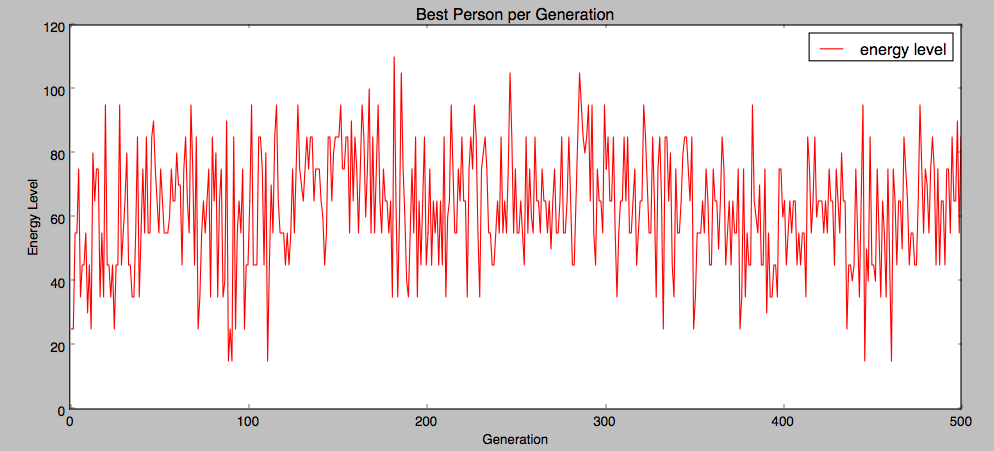
\includegraphics[width=1\textwidth]{40des_best}
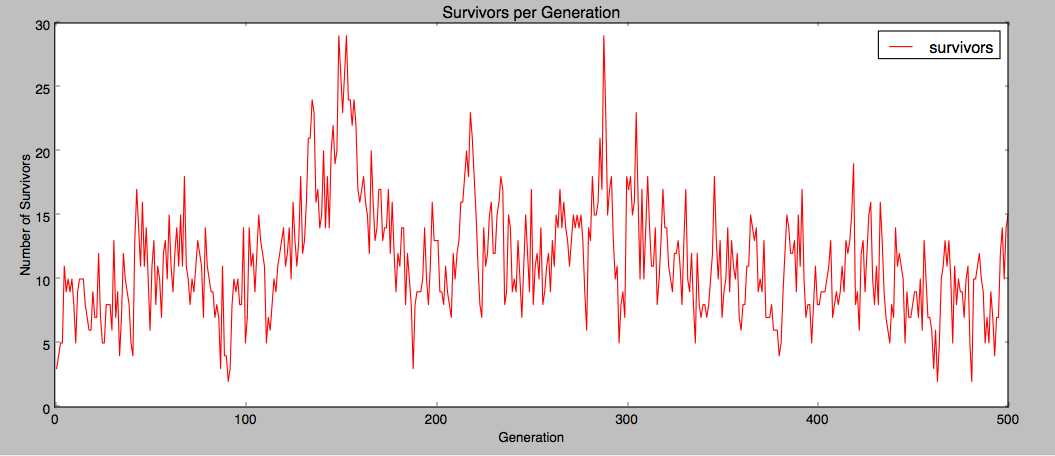
\includegraphics[width=1\textwidth]{40des_survivors}


%----------------------------------------------------------------------------------------
%	SECTION 3
%----------------------------------------------------------------------------------------

\section{Evolution's Effect and General Notes}

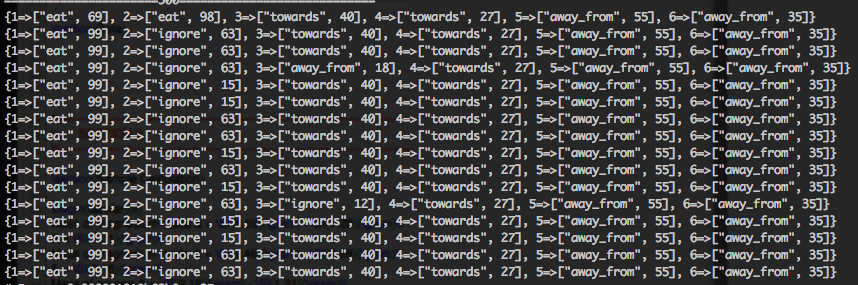
\includegraphics[width=1.35\textwidth,height=1.35\textheight,keepaspectratio]{15traits}\\ \\ \\ 
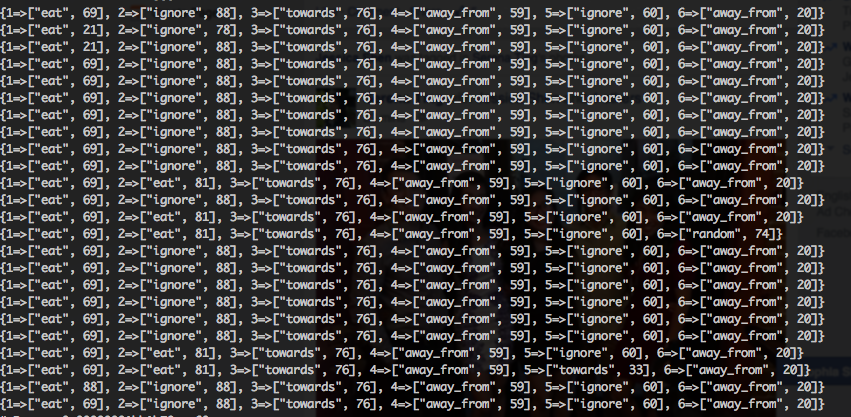
\includegraphics[width=1.35\textwidth,height=1.35\textheight,keepaspectratio]{40non_traits} \\ \\ \\
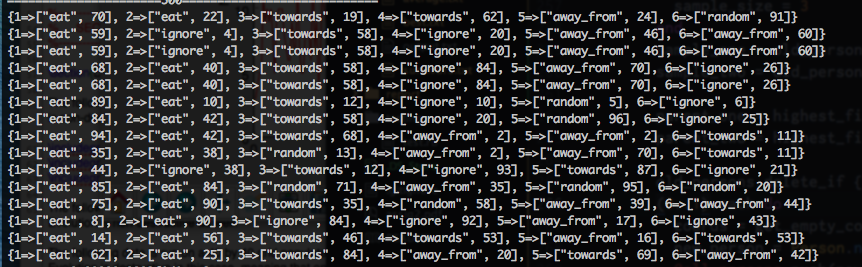
\includegraphics[width=1.35\textwidth,height=1.35\textheight,keepaspectratio]{40des_traits}
\\ \\ \\ 

It seems that non-destructive tournament selection returns a much higher survival rate with better genomes than destructive tournament selection (the third traits picture).  With non-destructive evolution, creatures tended to move towards having very similar chromosomes.  This happened mostly from some sort of bottle-neck effect, where if only 1 or 2 creatures were left, a very high portion of the next generation would be left with extremely similar genomes.  On the other hands, if only 1 or 2 creatures were left with destructive evolution, they would pass their genes on and a new batch of people with random chromosomes would populate the rest of the world.  Although non-destructive evolution had creatures with a higher survival rate and more energy, the destructive evolution returned generations with more variety, which could help in some unforeseen circumstance. \\ 

In general, after evolving for 500 generations, creatures tended to have higher weights on eating and moving towards strawberries, ignoring and moving away from mushrooms, ignoring and moving away from creatures, and a random selection of roles and weights for people (these didn't tend to matter since moving towards people didn't yield any benefits or costs).  \\ \\

\end{document}


